\section{Avaliação de Determinismo e Isolamento}

Para avaliar e validar o determinismo desse projeto, foi modelado um cenário onde o hipervisor seria utilizado em uma \gls{ecu} veícular. Para isso foram empregados quatro \gls{rtos} EPOS e um Linux
rodando uma atividades intensivas para tentar ao maximo gerar intrusividade.

As quatro instancias do EPOS rodam, cada uma, uma atividade diferente: Um dos EPOS roda um kalman filter em $5'000$ amostras, um roda uma convlução de um kernel $3\times3$ em uma imagem $512\times512$,
um roda transformada rápida de fourrier, e o outro roda conversão de coordenadas esféricas para coordenadas cartesianas em $50'000$ pontos.

Três das tarefas, com exeção do kalman filter, possuem uso intensivo de memória, em um cenário ideal, o objetivo desse experimento é observar uma variação nula ou mínima nesse, e uma maior nas outras
uma vez que a principal forma de interferencia é via cache de memória.

\begin{figure}[H]
\centering
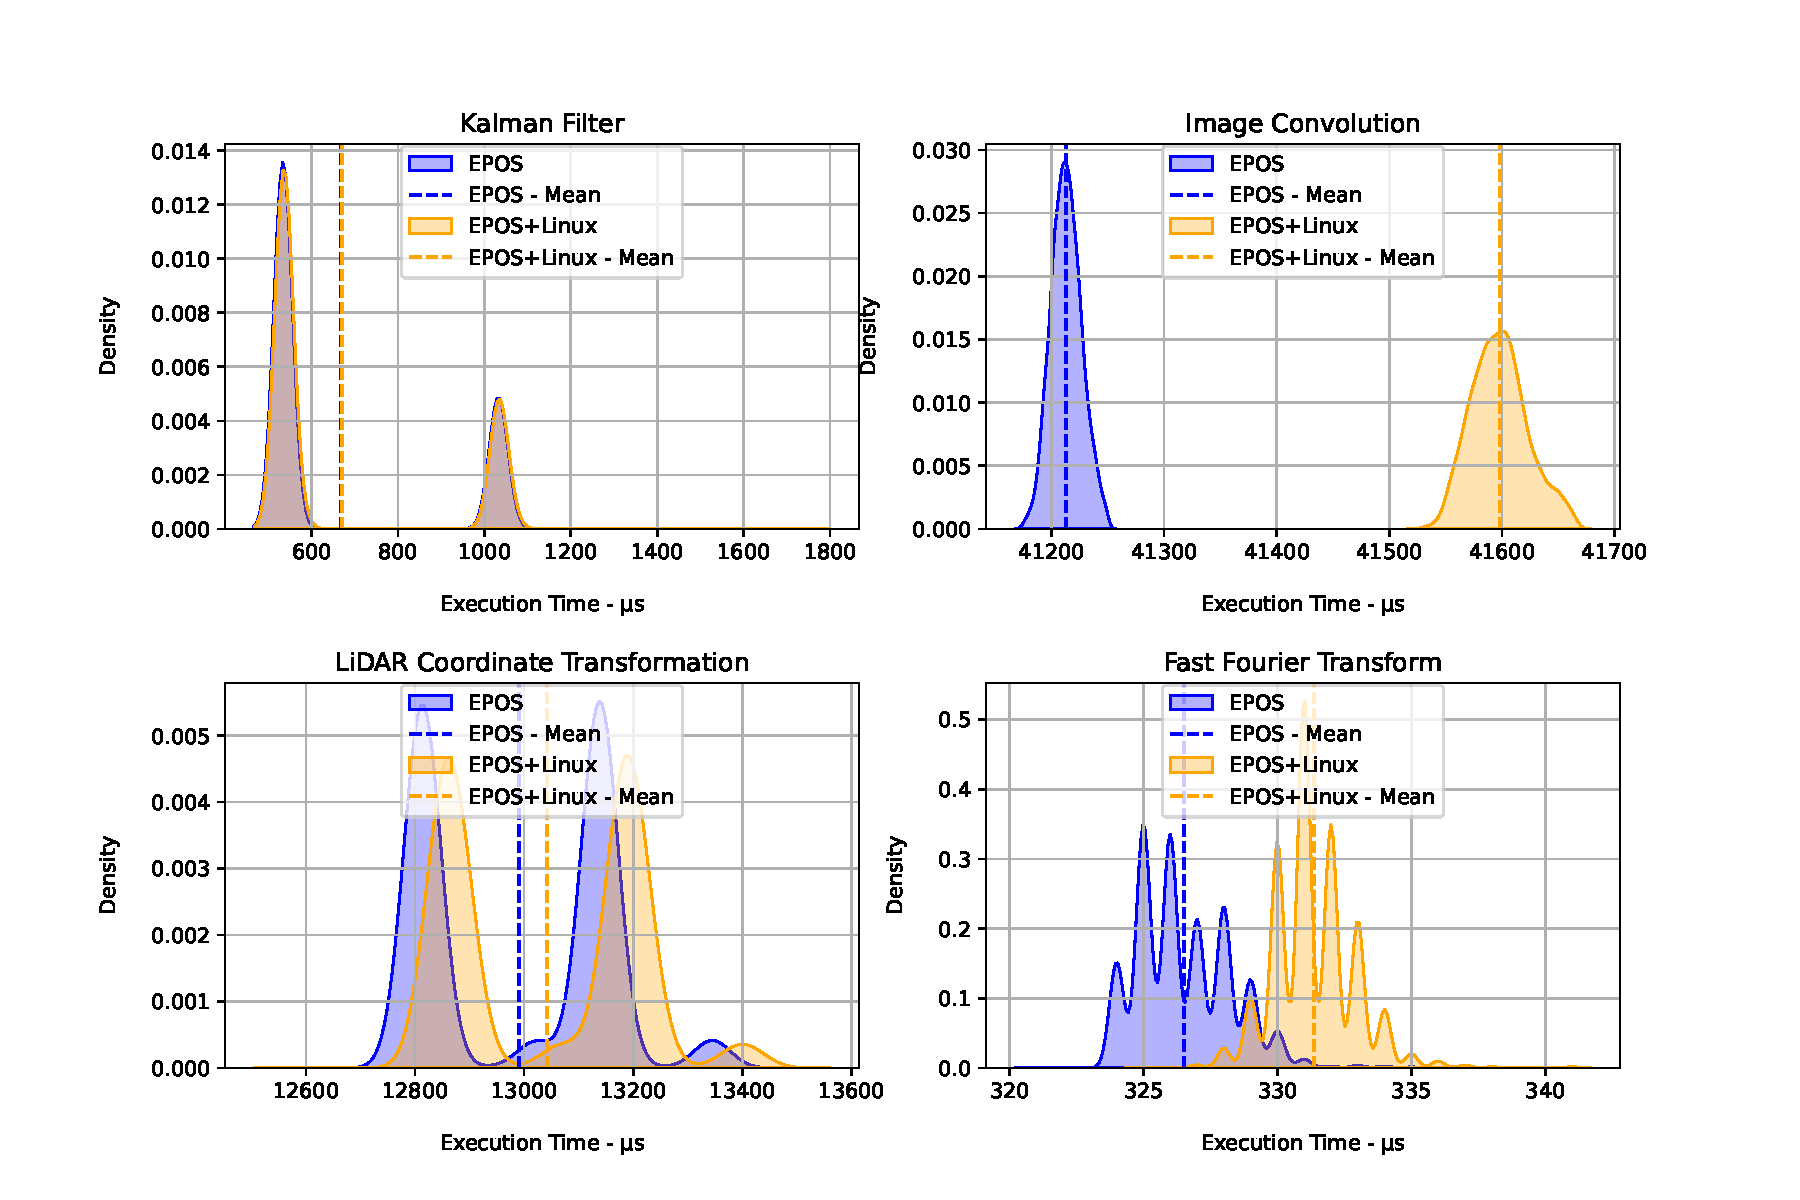
\includegraphics[width=1\textwidth]{images/VehicularBenchmarks.pdf}
\caption{Distribuição de Densidade dos Tempos de Execução das Tarefas do Cenário Veicular.}\label{fig:vehicular-benchmarks}
\end{figure}

\begin{table}[htbp]
    \centering
    \begin{tabular}{lrrrr}
        \toprule
        \textbf{Tarefa} & \textbf{EPOS ($\mu$)} & \textbf{EPOS ($\sigma$)} & \textbf{EPOS+Linux ($\mu$)} & \textbf{EPOS+Linux ($\sigma$)} \\ \midrule
        Kalman Filter   & 668,56 & 221,86 & 671,50 & 222,37 \\
        Convlução       & 41.212,63 & 17,37 & 41.597,71 & 29,89 \\
        Coordenadas     & 12.990,10 & 171,64 & 13.041,25 & 174,57 \\
        FFT             & 326,58 & 2,15 & 332,25 & 4,75 \\ \bottomrule
    \end{tabular}
    \caption{Comparação dos Tempos de Execução nos Cenários com e sem a Intrusividade do Linux.}\label{tab:vehicular-benchmarks}
\end{table}

A Figura~\ref{fig:vehicular-benchmarks} apresenta as distribuições de densidade probabilística para cada uma das instâncias do \gls{rtos}, avaliadas em isolamento e sob interferência do Linux
em segundo plano. Complementarmente, a Tabela~\ref{tab:vehicular-benchmarks} sintetiza a média e o desvio padrão obtidos nesses experimentos.

Como esperado, os resultados indicam que as tarefas com uso mais intensivo de memória foram as mais afetadas. Ainda assim, a interferência máxima manteve-se abaixo de $2\%$.

Para comprovar que a maior parte da interferência provém da memória, os dois cenários foram reavaliados com a ativação dos mecanismos de particionamento de cache da plataforma utilizada.
Esse mecanismo divide a cache em partes iguais para cada núcleo da CPU, amenizando a interferência mútua.

\begin{figure}[H]
\centering
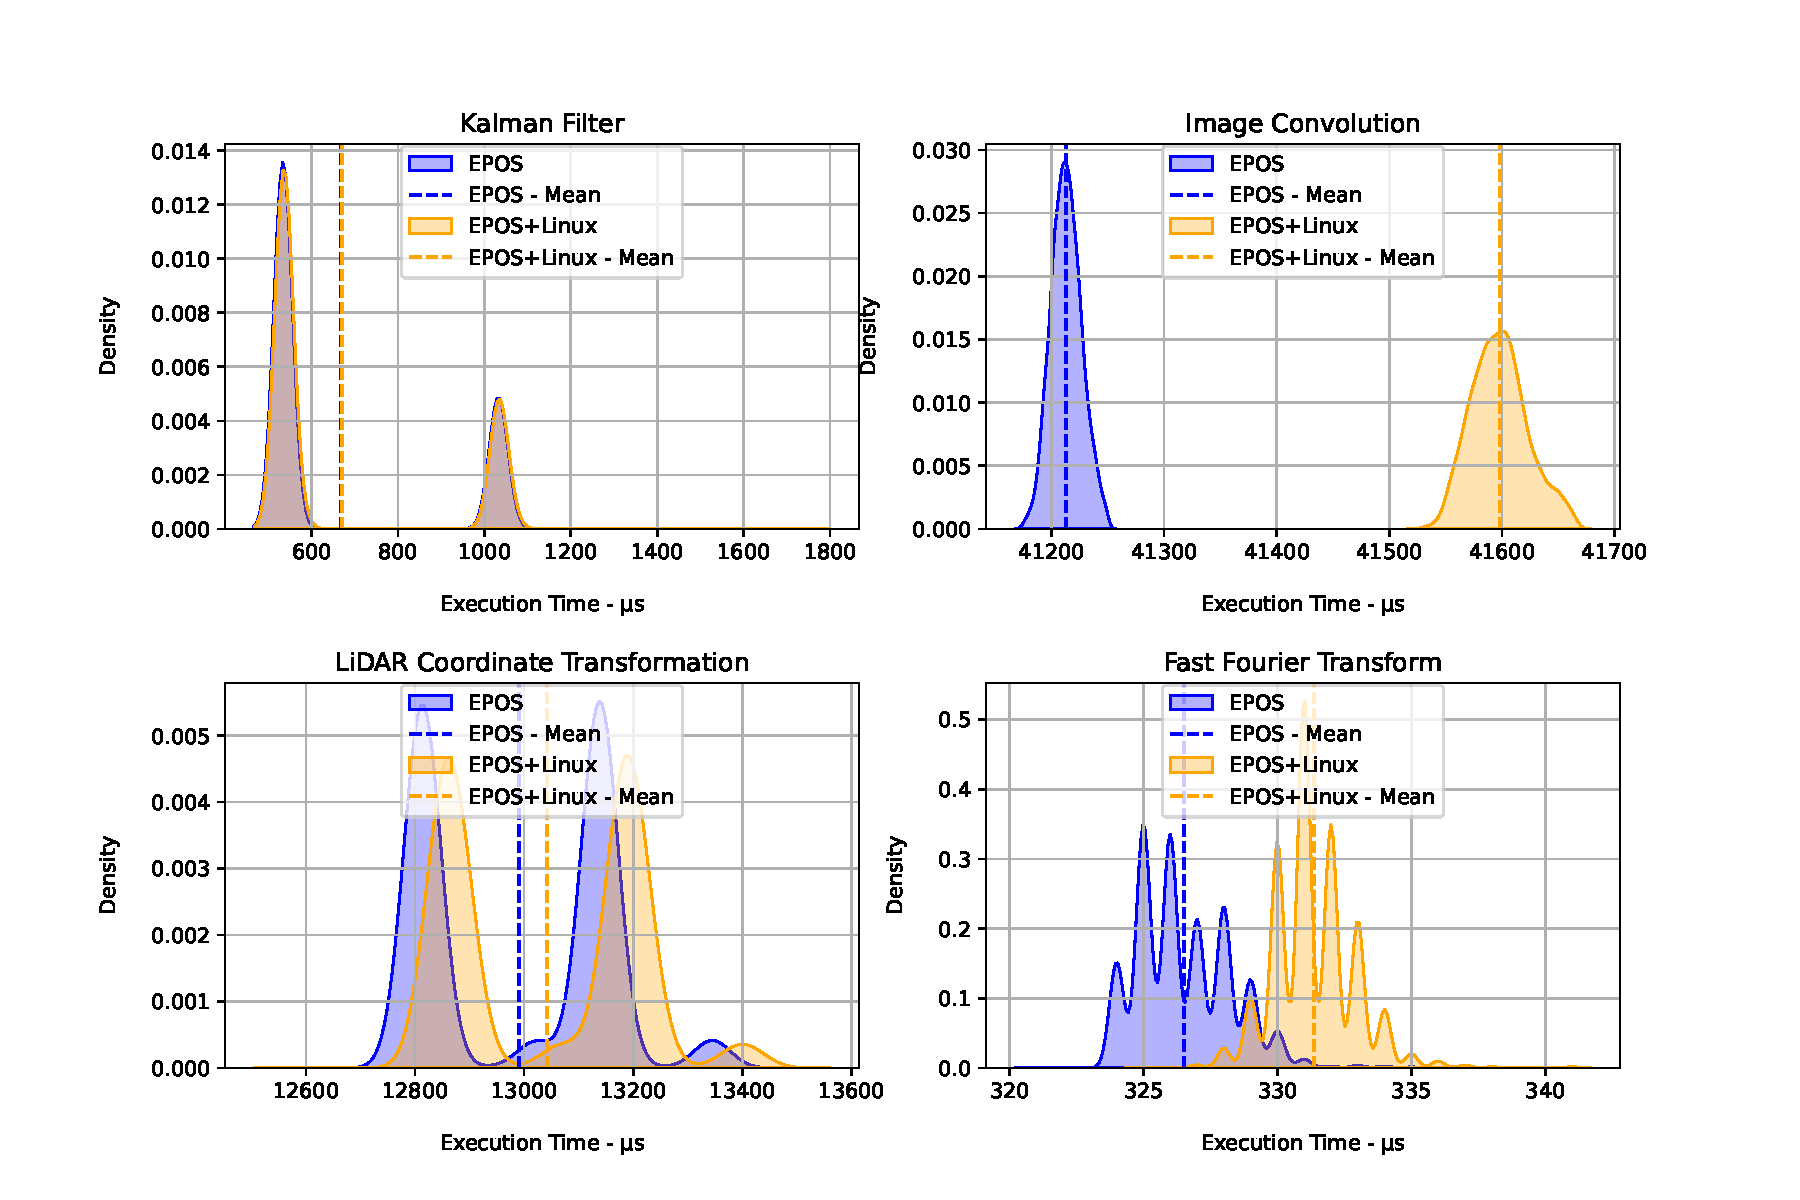
\includegraphics[width=1\textwidth]{images/VehicularBenchmarks.pdf}
\caption{Distribuição de Densidade dos Tempos de Execução das Tarefas do Cenário Veicular com Particionamento da Cache.}\label{fig:isolated-vehicular-benchmarks}
\end{figure}

\begin{table}[htbp]
    \centering
    \begin{tabular}{crrrr}
        \toprule
        \textbf{Tarefa} & \textbf{EPOS ($\mu$)} & \textbf{EPOS ($\sigma$)} & \textbf{EPOS+Linux ($\mu$)} & \textbf{EPOS+Linux ($\sigma$)} \\ \midrule
        Kalman Filter & $686{,}04$   & $230{,}87$ & $688{,}65$   & $230{,}92$ \\
        Convlução & $44\,630{,}28$ & $39{,}79$  & $45\,005{,}51$ & $50{,}90$  \\
        Coordenadas & $12\,844{,}28$ & $57{,}48$  & $12\,898{,}07$ & $58{,}02$  \\
        FFT & $327{,}10$   & $2{,}51$   & $331{,}41$   & $2{,}55$   \\
    \bottomrule
    \end{tabular}
    \caption{Comparação dos Tempos de Execução nos Cenários com e sem a Intrusividade do Linux com Particionamento da Cache.}\label{tab:isolated-vehicular-benchmarks}
\end{table}

O particionamento de cache reduz a interferência máxima para menos de 1,5\%, embora ainda persista uma parcela residual decorrente da competição no barramento de memória.


